
\begin{problem}{Gradient Calculation by Hand \hfill [10 pts]}{prob:handgrad}
\label{prob:handgrad}

Let's consider a very simple expression $L = (w_1 + w_2) \cdot w_3$. In this
expression, we can think of $w_1, w_2, w_3$ as parameters we can change, and $L$
as the result of this expression. If we told you $L$ was a loss function and
gave you the objective of minimizing loss, how would you choose your parameter
weights $w_i$? As covered in lecture, we can use \textit{gradient descent} (we
simplify it here)\ldots

\begin{itemize}
    \item Compute the rate of change of the result $L$ with respect to each
        parameter $w_i$. Since our expression for $L$ may have many variable
        parameters, we find the partial derivative denoted by $\frac{\partial
        L}{\partial w_i}$. We call this the \textit{gradient}. 
    \item Update our parameters via the rule $w_i \coloneq w_i -\eta
        \frac{\partial L}{\partial w_i}$ for some small learning rate $\eta$.
        There are different strategies for picking a learning rate (see
        lecture). This step moves each parameter $w_i$ in the direction opposite
        to the gradient.
    \item Repeat the above two steps until we converge to some $L^*$.
\end{itemize}

\begin{figure}[H]
    \centering
    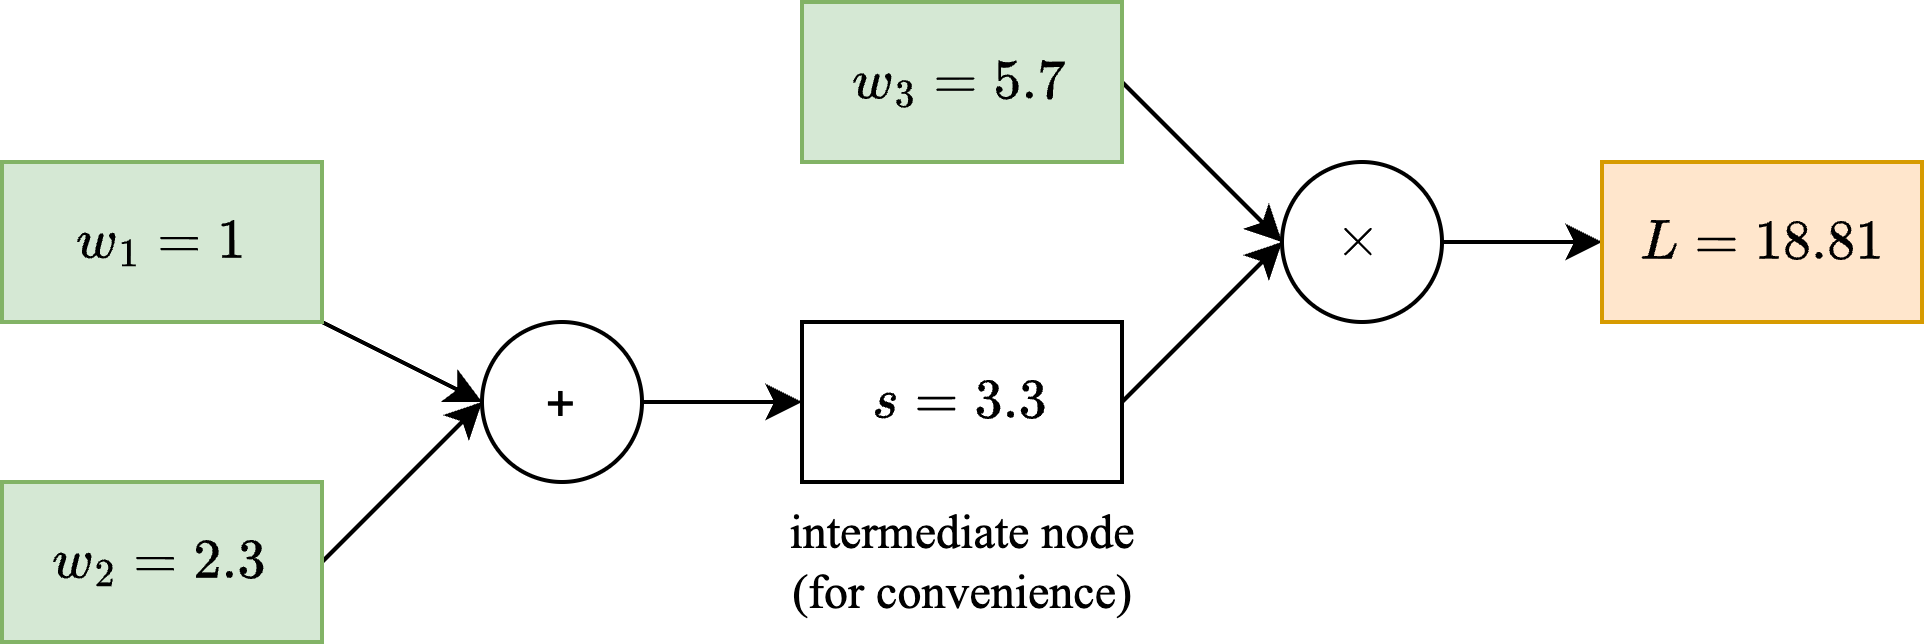
\includegraphics[width=0.7\linewidth]{media/hand_backprop.png}
    \caption{Expression diagram for $L$. We add intermediate node $s$ to
    represent the result of $w_1 + w_2$. This is a deliberate choice that'll
make more sense when we automate gradient backprop (next prob).}
    \label{fig:handbackprop}
\end{figure}

\begin{adjustwidth}{2em}{2em}
    
\textbf{(a)} \textbf{Calculate $\frac{\partial L}{\partial w_3}$.} \hfill (2 pts)

\begin{adjustwidth}{2em}{2em}
Please give an expression in terms of any of $w_1, w_2, w_3, s, L$. Then
plug in the values from \cref{fig:handbackprop} to get a value. We'll look
for both the expression and final value.\\
\end{adjustwidth} 
\vspace{5px}

\textbf{(b)} \textbf{Calculate $\frac{\partial L}{\partial w_1}$ and
$\frac{\partial L}{\partial w_2}$.} \textit{hint: use chain rule} \hfill (2
pts)
\begin{adjustwidth}{2em}{2em}
Your expressions must contain $\frac{\partial s}{\partial w_1}$ or
$\frac{\partial s}{\partial w_2}$. Evaluate using values from
\cref{fig:handbackprop}. \\
\end{adjustwidth} 
\vspace{5px}

\textbf{(c)} \textbf{Update parameters} \hfill (4 pts)
\begin{adjustwidth}{2em}{2em}
    Now with learning rate $\eta = 0.01$, calculate the new parameter values
    $w_1, w_2, w_3$ after one step. Notice that we calculate all the
    gradients first, then update all of the parameters. We will follow this
    order when we automate everything in problem 2.\\ 
\end{adjustwidth}

\textbf{(d)} \textbf{Analysis} \hfill (2 pts)
\begin{adjustwidth}{2em}{2em}
    Using the newly updated parameter values, calculate the new result value
    of $L$ and compare it with the original value. What do you expect? What
    do you see? Did $L$ increase or decrease?
\end{adjustwidth}
\end{adjustwidth}

\end{problem}

\begin{solution*}{}{}
\textbf{(a)} Since $L = w_3 \cdot s = w_3 \cdot (w_1 + w_2)$,

\[
\frac{\partial L}{\partial w_3} = (w_1 + w_2) = 1 + 2.3 = 3.3
.\] 

\textbf{(b)} Since $L = w_3 \cdot s$ and $s = (w_1 + w_2)$,

\[
\frac{\partial L}{\partial w_1} = 
\frac{\partial L}{\partial s} \cdot \frac{\partial s}{\partial w_1}  = 
w_3 \cdot \frac{\partial (w_1 + w_2)}{\partial w_1} = 
w_3 \cdot 1 = w_3 = 5.7
.\] 

Using the same logic for $w_2$,

\[
\frac{\partial L}{\partial w_2} = 
\frac{\partial L}{\partial s} \cdot \frac{\partial s}{\partial w_2}  = 
w_3 \cdot \frac{\partial (w_1 + w_2)}{\partial w_2} = 
w_3 \cdot 1 = w_3 = 5.7
.\] 
\vspace{5px}

\textbf{(c)} 

\begin{align*}
    w_1 &\to w_1 - \eta \cdot \frac{\partial L}{\partial w_1} = 1 - 0.01 \cdot
    5.7 = 0.943 \\ 
    w_2 &\to  w_2 - \eta \cdot \frac{\partial L}{\partial w_2} = 2.3 - 0.01 \cdot
    5.7 = 2.243 \\ 
    w_3 &\to w_3 - \eta \cdot \frac{\partial L}{\partial w_3}  = 5.7 - 0.01 \cdot
    3.3 = 5.667
.\end{align*}

\textbf{(d)} \textbf{Analysis} \hfill (2 pts)
\begin{adjustwidth}{2em}{2em}
Using the newly updated parameter values, calculate the new result value
of $L$ and compare it with the original value. What do you expect? What
do you see? Did $L$ increase or decrease?
\end{adjustwidth}

\[
L = (w_1 + w_2) \cdot w_3 = (0.943 + 2.243) \cdot 5.667 = 18.055062
.\] 

The loss should decrease, and it did in fact decrease.
\end{solution*}
